\chapter{First Order Differential Equations}
\section{Modeling and Differential Equations}
You may recall that in an algebraic equation you are seeking to find a number,
usually\footnote{See the TED Talk
    \href{https://www.ted.com/talks/terry_moore_why_is_x_the_unknown}{https://www.ted.com/talks/terry\_moore\_why\_is\_x\_the\_unknown}
to see why we use $x$ for the unknown in Algebra.}
$x$, so that the given equation holds true.  For example, we could solve $x+2 = 5$ and
find that $x=3$ is the only value that makes the equal sign true.  As another example, we
could solve $x^2-3x+2 = 0$ using the quadratic formula or factoring and find that $x=1$
and $x=2$ are the only solutions. Your high school algebra classes focused on the
techniques necessary to solve many different types of algebraic equations and at this
point you likely have the techniques down pat (right?!).

When solving differential equations we are seeking a slightly different goal.  This time
the unknown is a function and the equation relates the derivative(s) of the function to
the function itself.  For example, if we consider the simple equation $y'(t) = y(t)$ we could
probably guess (using the rules of calculus) that the only functions that satisfy this
equation are $y(t) = 0$ and $y(t) = Ce^t$.  Notice that the solution is not a number but a
function.  As another example consider $y''(t) = -y(t)$.  In this case you can also use
your intuition from calculus to guess that $y(t)$ is some combination of sines and
cosines: $y(t) = C_1 \sin(t) + C_2 \cos(t)$. Our goal throughout this course is to build
differential equations and find techniques to analyze them. As you might imagine based on
the complexity of the derivative rules in calculus, the techniques to find solutions to
differential equations can sometimes be quite complicated.

\begin{definition}[Differential Equation]
    A {\bf differential equation} is an equation that relates a function to its
    derivative(s).  The goal in solving a differential equation is to find the function
    that satisfies the given relationship.
\end{definition}

Let's begin by examining a few modeling-type problems where you need to write the
differential equation.  After we have a few differential equations we will spend some time
building up the basic solution techniques. \\
Note: You are expected to have seen several of these techniques already.  If these notes
move to fast then go to the appropriate linked texts in Section \ref{pref:resources}.

\begin{problem}%www.simiode.org Problem 1-001pgf-T-BirthDeathImmigration
    Write a differential equation for each of the following situations.  Let $P(t)$ be a
    function representing the population at time $t$ (measured in years).  To help you write each differential equation think
    about answering the question: \\
    {\it How does the rate of change of the population relate to the size of the population?}
    \begin{enumerate}
        \item[(a)] A fragile population has a 50\% chance of surviving in any given year.  
        \item[(b)] The same fragile population simultaneously has an influx of 10 new
            members every year.
        \item[(c)] The population in parts (a) and (b) has a reproduction rate of 15\%
            each year (measured after the immigrants arrive).
    \end{enumerate}
\end{problem}
\solution{
    \begin{enumerate}
        \item[(a)] $P'(t) = -0.5P$
        \item[(b)] $P'(t) = -0.5P + 10$
        \item[(c)] $P'(t) = 0.15\left( -0.5P + 10 \right)$
    \end{enumerate}
}

\begin{problem}\label{prob:ice_balls}
    Did you know that you could make spherical ice cubes \ldots wait, that name seems
    wrong \ldots whatever, check out
    \href{https://www.amazon.com/Tovolo-Sphere-Ice-Molds-Set/dp/B007ACTN54}{THIS LINK}.
    I have several questions.
    \begin{enumerate}
        \item[(a)] Finish this sentence: 
            \begin{quote}
                The rate of change of the volume of the ice ball is proportional to
                \underline{\hspace{1in}}
            \end{quote}
        \item[(b)] Write your answer from part (a) as a differential equation.  Be sure
            that the left-hand and right-hand sides of your differential equation refer to
            the same variables.
        \item[(c)] I want to know which type of ice will keep my drink cold longer:
            sphere-shaped or cube-shaped.  Assume that both chunks of ice start with
            exactly the same volume.  What differential equations would you need to solve
            to answer this question?
    \end{enumerate}
\end{problem}
\solution{
    \begin{enumerate}
        \item[(a)] The rate of change of the volume of the ice ball is proporitonal to the
            surface area of the ice ball.
        \item[(b)] At first we could write $\frac{dV}{dt} = k S$ where $S$ is the surface
            area, but knowing that the surface area of a sphere is $S = 4\pir^2$ and the
            volume is $V = \frac{4}{3} \pi r^3$ we can solve for $r$ in the volume formula
            and substitute into the surface area to get
            \[ r = \sqrt[3]{\frac{3}{4\pi} V} \quad \implies \quad S = 4 \pi \left(
            \frac{3}{4\pi} V
        \right)^{2/3}. \]
        Therefore the differential equation is
        \[ \frac{dV}{dt} = 4 \pi k \left( \frac{3}{4\pi} V \right)^{2/3}. \]
    \item[(c)] Finally, the differential equation for the cube is simpler (since the
        geometry is simpler) so $S = 6 x^2$ and $V = x^3$ where $x$ is the length of a
        side of the cube.  Therefore, $x = V^{1/3}$ and $S = 6 V^{2/3}$ and 
        \[ \frac{dV}{dt} = 6 V^{2/3}. \]
    \end{enumerate}
}

\begin{problem}
An ant is building a tunnel.  We want to create a differential equation model for the
total time that it takes for the ant to build the tunnel as a function of the length of
the tunnel.  Which of the following would be an appropriate differential equation? Let $x$
be the length of the tunnel and let $T(x)$ be the total time to dig a tunnel of length
$x$.  
% 
% Use what you know about calculus to find a solution for every one of the following
% proposed models and use your solution to help decide which is the correct model.
\begin{enumerate}
    \item $T' = kT$ (rate of change of time proportional to total time taken)
    \item $T' = kx$ (rate of change of time proportional to current length of the tunnel)
    \item $T' = kx^3$ (rate of change of total time proportional to volume). 
    \item $T' = kS$ (rate of change of total time proportional to the surface area of the end of
the tunnel)
\end{enumerate}
\end{problem}
\solution{
$T' = kx$ (rate is proportional to length of tunnel).
\[ T'=kx \iff T(x) = \frac{k}{2}x^2 \]
So the time that it takes to dig the tunnel is a quadratic function of the length. \\
Show a slope field with $T(0)=0$ and various values of $k$.
}



\begin{problem}
    A population of Alaskan Salmon grows according to the following rules:
    \begin{itemize}
        \item If there are no salmon then the population doesn't change (duh).
        \item If the population reaches the carrying capacity for the environment, $M$,
            the size of the population stops changing.
        \item When the population is growing and is far away from the carrying capacity
            the growth rate is roughly proportional to the size of the population.
    \end{itemize}
    Write a differential equation that models this scenario.  Support your model by
    discussing what occurs when $P$ is close to $M$ and when $P$ is close to $0$.
    \[ \frac{dP}{dt} = \underline{\hspace{2in}} \]
\end{problem}
\solution{
    \[ \frac{dP}{dt} = kP \left( 1-\frac{P}{M} \right) \quad \text{or} \quad
    \frac{dP}{dt} = kP \left( M-P \right) \]
    Note that the units of $k$ are different in the two proposed solutions.
}

\begin{problem}
    A spring oscillates in such a way that its acceleration is proportional to its
    position relative to an equilibrium point.
    \begin{itemize}
        \item If the spring is a long way from equilibrium then the acceleration is large
            and pointed back toward equilibrium.
        \item If the spring is close to equilibrium then the acceleration is small.
    \end{itemize}
    Let $y(t)$ be the position of the spring.
    \[ \frac{d^2 y}{dt^2} = \underline{\hspace{2in}} \]
    Sketch a plot of the solution to this differential equation.
\end{problem}
\solution{
    \[ \frac{d^2 y}{dt^2} = -ky \]
}


\newpage
\section{Differential Equation Terminology}
In this chapter we will look at a few techniques for solving first-order differential
equations.  Before launching to the techniques let's get a little bit of terminology on
the table.  I am expecting that much of this terminology is familiar to you already from
previous classes. We are going to cover this very quickly and we will be leaving some of
the reading and remembering up to you.

\begin{definition}[First Order Differential Equation]
    A {\bf first order differential equation} is a differential equation of the form 
    \[ y'(t) = f(y,t). \]
    Notice that a first order differential equation contains only the first derivative of
    the unknown function (hence the name).  The function $f$ can be just about anything
    and it depends on both $y(t)$ and maybe $t$ explicitly.
\end{definition}

\begin{definition}[Autonomous Differential Equation]
    An {\bf autonomous differential equation} is a differential equation of the form
    \[ y'(t) = f(y) \]
    where there is no explicit dependence of the independent variable $t$ on the
    right-hand side of the equation. A differential equation that has explicit dependence
    on $t$ is called {\bf non-autonomous}.  
\end{definition}
To clarify this point consider the following examples:
\begin{flalign}
    \text{first order autonomous D.E:} \quad & y'(t) = -0.2y(t) + 4 \\
    \text{first order non-autonomous D.E:} \quad & y'(t) = -0.2y(t) + 4t 
\end{flalign}

\begin{definition}[Linear First Order Differential Equation]
    A {\bf linear} first order differential equation has the form
    \[ y'(t) + P(t) y(t) = Q(t) \qquad \text{or} \qquad y'(t) = -P(t) y(t) + Q(t). \]
    The reason for the name ``linear'' is that the right-hand side of this equation is
    literally a linear function of $y$.  Hence the differential equation can be written as
    $y' = f(y)$ where $f(y) = -Py + Q.$
\end{definition}

\begin{definition}[Homogenous Differential Equations]
    A differential equation is called {\bf homogeneous} if, loosely speaking, no terms appear
    that do not involve the unknown function.  Another way to say this is that every term
    in the differential equation will either contain the function $y(t)$ or its
    derivatives.  A differential equation that is not homogeneous is called {\bf
    non-homogeneous}.
\end{definition}
\begin{problem}
    It is often a good exercise to make examples associated with new definitions.  For
    each of the above definitions create an example of a differential equation that {\it
    is} described by the definition and a differential equation that {\it is not}
    described by the definition.
\end{problem}

\begin{problem}
    Come up with an example for each of the following descriptions of differential
    equations.
    \begin{enumerate}
        \item[(a)] A linear first order homogeneous differential equation.
        \item[(b)] A non-linear first order homogeneous differential equation.
        \item[(c)] A linear first order non-autonomous differential equation.
        \item[(d)] A linear first order non-autonomous differential equation that is
            homogeneous.
        \item[(e)] A linear first order non-autonomous differential equation that is
            non-homogeneous.
    \end{enumerate}
\end{problem}
\solution{
    \begin{enumerate}
        \item[(a)] $y'=-0.2y$ 
        \item[(b)] $y'=-0.2y^2$ 
        \item[(c)] $y'=-0.2y+t$ 
        \item[(d)] $y'=-0.2yt$ 
        \item[(e)] $y'=-0.2y+3t$ 
    \end{enumerate}
}
\begin{example}
    Here are a few examples of homogeneous and non-homogeneous differential equations.
    \begin{itemize}
        \item The differential equation $y' = -0.2y$ is homogeneous.
        \item The differential equation $y' = -0.2y + 3$ is non-homogeneous.
        \item The differential equation $y'' + 3y' - 5y = 0$ is homogeneous.
        \item The differential equation $y'' + 3y' - 5y = 2$ is non-homogeneous.
        \item The differential equation $v' = g - c v^2$ is non-homogeneous (and
            nonlinear).
    \end{itemize}
\end{example}

\newpage
\section{Solution Technique: Integration}
In the sections that follow we will review (or introduce) some of the primary solution
techniques for first order differential equations.  As has been mentioned before, it is
likely that you have seen these techniques before but it is worth your time to blow the
dust off of your memories and to review what you once knew.  

\begin{problem}
    For each of the following differential equations use the rules of Calculus find the
    function $y(t)$ that solve the differential equation.
    \begin{flalign*}
        \frac{dy}{dt} &= 2t + 5 \quad \text{with} \quad y(0) = 3 \\
        \frac{dy}{dt} &= \sin(t) \quad \text{with} \quad y(0) = 1 \\
        \frac{dy}{dt} &= t e^{-t^2} \quad \text{with} \quad y(0) = 0 \\
    \end{flalign*}
\end{problem}
\solution{
    \begin{flalign*}
        y(t) &= t^2 + 5t + 3 \\
        y(t) &= -\cos(t) + 2 \\
        y(t) &= -\frac{1}{2} e^{-t^2} + \frac{1}{2}
    \end{flalign*}
}

\begin{technique}[Solution via Integration]
    To solve
    \[ \frac{dy}{dt} = f(t) \]
    you can first think of ``multiplying by $dt$'' to get $dy = f(t) dt$.  Then integrate both
    sides with respect to $t$. Therefore, $y(t) = \int f(t) dt + C = F(t) + C$ where $F(t)$ is
    the antiderivative of $f(t)$ such that $F'(t) =
    f(t)$.  Given $y(t_0) = y_0$ we can get $C$ by
    \[ y_0 = F(t_0) + C \quad \implies \quad C = y_0 - F(t_0) \]
\end{technique}

\begin{problem}
    Create and solve a first order differential equation (along with an appropriate initial
    condition) that can be solved using the technique of integration.
\end{problem}

\begin{problem}
    Solve the differential equation
    \[ y'(t) = e^{-2t} \quad \text{with} \quad y(0) = 1 \]
\end{problem}
\solution{
    \[ y(t) = \int e^{-2t} dt = -\frac{1}{2} e^{-2t} + C \]
    \[ y(0)=1 \implies 1 = -\frac{1}{2} + C \implies C = \frac{3}{2} \implies y(t) =
    -\frac{1}{2} e^{-2t} + \frac{3}{2} \]
}

\begin{problem}
    A stone is dropped from rest at an initial height $h$ above the surface of the earth.
    We want to show that the speed with which it strikes the ground is $v = \sqrt{2gh}$.
    Start by writing an appropriate differential equation and then use the
    differential equation to very this result. You do not need to include air resistance
    in your model.
\end{problem}
\solution{
    \[ \frac{dv}{dt} = -g \implies v(t) = -gt + 0 \implies \frac{dy}{dt} = -gt \implies
    y(t) = -\frac{gt^2}{2} + h \implies t_{ground} =\sqrt{\frac{2h}{g}} \]
    Therefore,
    \[ v_{ground} = -g\sqrt{\frac{2h}{g}} = -\sqrt{2gh} \]
}

\newpage
\section{Solution Technique: Separation of Variables}
\begin{problem}
    Consider the differential equation 
    \[ \frac{dy}{dt} = y \]
    with the initial condition $y(0) = 1$.
    \begin{enumerate}
        \item[(a)] Putting the differential equation into words: \\ {\it the derivative of
            some unknown function is equal to the function itself.} \\
            what is the function?
        \item[(b)] Allow me to abuse some notation: \\
            If you multiply both sides by $dt$ and divide both sides by $y$ we end up with
            \[ \frac{dy}{y} = dt. \]
            Integrate both sides and solve for $y$.
        \item[(c)] Compare your answers to parts (b) and (c).
    \end{enumerate}
\end{problem}
\solution{
The solution is clearly $y(t) = e^t$.
}

\begin{problem}
    In part (b) of the previous problem I said that I was ``abusing notation''.  What does
    that mean?  What notation is being abused?
\end{problem}

\begin{technique}[Separation of Variables]
    To solve a differential equation of the form
    \[ \frac{dy}{dx} = f(y)\cdot g(x) \]
    Separate and integrate by treating the ``$dy/dt$'' as a fraction\footnote{Technically
        speaking the ``$dy/dt$'' is not a fraction it is a shorthand notation for a
    limit.  More technically there is some sneaky chain rule happening behind the scenes
here \ldots can you find it.}
    \[ \int \frac{dy}{f(y)} = \int g(x) dx \]
    Notice that the right-hand side of the differential equation factors perfectly hence
    separating the variables into the functions $f$ and $g$.
\end{technique}

\begin{problem}
    With your partner, write a differential equation that can be solved via separation of
    variables.  Once you have your equation trade with a different group and solve their
    equation.
\end{problem}

\begin{problem}
    A drug is eliminated from the body via natural metabolism.  Assume that there is an
    initial amount of $A_0$ drug in the body.  Which of the following is the best
    differential equation model for the drug removal?  Once you have the model solve it
    with the appropriate technique.
    \begin{enumerate}
        \item $A' = -kt$
        \item $A' = -kA$
        \item $A' = -kA(1-A/N)$
        \item $A' = -kAt$
    \end{enumerate}
\end{problem}
\solution{
    $A'=-kA$ so $A(t) = Ce^{-kt}$ with separation of variables.  \\ Show a slope field for
    this and discuss stability and equilibrium. Also discuss why the other won't work.
}

\begin{problem}
    In a dog, an intravenous dose of 30 mg of pentobarbital sodium per kilogram of body
    weight will usually produce surgical anesthesia. Also in the dog, pentobarbital has a
    biological halflife of about 4.5 hours, due almost entirely to metabolism.  You
    anesthetize a 14-kg dog with the above dose of pentobarbital. Two hours later the
    anesthesia is obviously beginning to lighten and you want to restore the original
    depth of anesthesia. How many milligrams of pentobarbital sodium should you inject?
    Write and solve a differential equation to answer this question.
\end{problem}
\solution{
    The simplest differential equation model is 
    \[ \frac{dP}{dt} = -kP \]
    where $P$ is the amount of pentobarbital (in mg) and $t$ is time (in hours).  The
    solution is clearly $P(t) = C e^{-kt}$ where $C = 420 = (14 \text{kg})(30
    \text{mg/kg})$.  Since we know the half life of the drug we can find $k$ as
    \[ 0.5P_0 = P_0 e^{-k(4.5)} \quad \implies \quad k \approx 0.154033 \]
    and hence $P(t) = 420 e^{-0.15033t}$.
}


\begin{problem}
    In a local pine forest the Pine Beetle is killing the trees at a rate proportional to the
    number of available trees in the forest.  A conservation group is attempting to curb the
    problem by planting 5 live trees per week.  Write a differential equation describing
    this scenario, classify the differential equation, and determine if it can be solved
    with separation of variables.
%     Which of the following is a mathematical model
%     for the number of live trees as a function of time (measured in weeks)?
%     \begin{enumerate}
%         \item $T' = -kT + 5$
%         \item $T' = -kT + 5*t$
%         \item $T' = -5k*T*t$
%         \item $T' = -5k*t$
%     \end{enumerate}
\end{problem}
\solution{
$T' = -kT + 5$.  First order, linear, autonomous, non-homogeneous. Separation is fine
since is it autonomous.
\[ \int \frac{dT}{T-5/k} = \int -k dt = -kt+C \implies \ln(T-5/k) = -kt+C \implies T =
Ce^{-kt} + \frac{5}{k} \]
}


\begin{problem}
    True or False: Every first order autonomous differential equation is separable. Be
    able to defend your answer.
\end{problem}
\solution{True, but the integration may be horrible!}


\begin{problem}
    In the movie Interstellar, ``Plan B'' was for the astronauts to start a colony on a new
    planet.  There was 1 female in the group so she would presumably carry the children.
    Genetic diversity was no problem because of the donor eggs.  The supplies on the colony
    would be limited by local resources as well as what they brought with them
    (which minimal).  Which of the following models should the astronauts use to plan
    their future reproduction, and what do the parameters mean?  Explain your choice for the best one.
    \begin{itemize}
        \item $P' = kP$
        \item $P' = kt$
        \item $P' = -kP\ln(P/N)$
        \item $P' = kP(1-P/N) $
    \end{itemize}
\end{problem}
\solution{A logistic model is the best choice. Either of the last two choice could work.
    \[ \int \frac{dP}{P\ln(P/N)} = \int -k dt \implies \int \frac{dP}{P\ln(P/N)} = -kt + C
    \]
    \[ \implies (\text{with } u=P/N) \,  \int \frac{1}{u\ln(u)} = -kt+C \implies
    (\text{with } v=1/u) \, \int \frac{1}{v}dv = -kt + C \]
    \[ \implies \ln(v) = -kt+c \implies \ln(\ln(P/N))=-kt+C \implies \ln(P/N) = Ce^{-kt}
    \implies P(t) = N e^{Ce^{-kt}} \]

    For the more standard logistic model:
    \[ \int \frac{dP}{P(1-P/N)} = -kt+C \implies \int \frac{A}{P} + \frac{B}{1-P/N} dP =
    -kt + C \implies \int \frac{1}{P} + \frac{(1/N)}{1-P/N} dP = -kt+ C \]
    \[ \implies \ln(P) - \ln(1-P/N) = -kt+C \implies \ln \left( \frac{P}{1-P/N} \right) =
    -kt+C\]
    \[ \implies \frac{P}{1-P/N} = Ce^{-kt} \implies P(t) = \frac{Ce^{-kt}}{1-Ce^{-kt}/N}
    \]

}


\newpage\section{Solution Technique: Undetermined Coefficients}
Some folks call this technique the ``four step method'', but in reality this is just one
of many techniques for solving non-homogeneous differential equations.  Instead of
thinking of this in ``four steps'' you should really just consider this a bit of
mathematical detective work.  

\begin{technique}[Solving Non-Homogeneous Differential Equations]
    The method of {\it undetermined coefficients} is roughly outlined as:
    \begin{enumerate}
        \item find a solution for the homogeneous differential equation,
        \item conjecture a particular solution for the non-homogeneous differential equation, 
        \item use the initial condition to find a relationship between some of the
            coefficients, and
        \item use the particular solution in the differential equation to find the
            remaining coefficients.
    \end{enumerate}
\end{technique}

\begin{problem}
    Solve the following first order linear non-homogeneous differential equation by
    following the steps outlined.
    \[ \frac{dy}{dt} = -0.2 y + 3 \quad \text{with} \quad y(0) = 5 \]
    \begin{enumerate}
        \item First solve the homogeneous part of the equation using separation of
            variables: $y' = -0.2y$.
            \[ y_{hom}(t) = \underline{\hspace{1in}} \]
            \solution{$y_h(t) = C_0 e^{-0.2t}$}
        \item Next conjecture that a {\it particular} solution has the same functional
            form as the non-homogeneity.  In this case the non-homogeneity is a constant
            function so we guess that the particular function is a generic constant
            function
            \[ y_{particular}(t) = C. \]
        \item The full analytic solution to the differential equation is the sum of the
            homogeneous and particular solutions: $y(t) = y_{hom}(t) + y_{part}(t)$.  Note
            that this is only the case for linear differential equations.
            \[ y(t) = \underline{\hspace{2in}} \]
            \solution{$y(t) = C_0 e^{-0.2t} + C_1$}
        \item Substitute the particular solution into the differential equation and see
            what equation comes out
            \[ \underline{\hspace{1in}} = \underline{\hspace{1in}} \]
            \solution{$0=-0.2C_1+3 \implies C_1 = 3/0.2=15$ }
        \item Substitute the initial condition into the analytic solution and see what
            equation comes out
            \[ \underline{\hspace{1in}} = \underline{\hspace{1in}} \]
            \solution{$5=C_0 + 15 \implies C_0 = -10$ }
        \item Determine the final solution
            \solution{$y(t) = -10e^{-0.2t} + 15$}
    \end{enumerate}
\end{problem}


\begin{technique}[Undetermined Coefficients]
    To solve a non-homogenous linear differential equation:
    \begin{enumerate}
        \item Solve the associated homogeneous differential equation.
        \item Conjecture a {\it particular solution} that has the same functional form as
            the non-homogeneity.
        \item Build the full analytic solution as a linear combination of the homogeneous and
            particular solutions: $y(t) = y_{hom}(t) + y_{part}(t)$.
        \item Substitute the particular solution into the differential equation.
        \item Subsitute the intitial condition(s) into the analytic solution.
        \item Use the equations that you found in steps 4 and 5 to find the constants.
    \end{enumerate}
\end{technique}

\begin{problem}\label{prob:undet_coeff}
    For each of the following linear non-homogeneous differential equations write the homogeneous solution and the particular solution. 
    \begin{enumerate}
        \item[(a)] $y' = 3y + 4$ \qquad $y_{hom}(t) = \underline{\hspace{1in}}$\, and\, $y_{part}(t) = \underline{\hspace{1in}}$
        \item[(b)] $y' = 3y + 4t$\qquad $y_{hom}(t) = \underline{\hspace{1in}}$\, and\, $y_{part}(t) = \underline{\hspace{1in}}$
        \item[(c)] $y' = 3y + 4\sin(t)$\qquad $y_{hom}(t) = \underline{\hspace{1in}}$\,
            and\, $y_{part}(t) = \underline{\hspace{1in}}$
        \item[(d)] $y' = 3y + 4e^{-t}$\qquad $y_{hom}(t) = \underline{\hspace{1in}}$\,
            and\, $y_{part}(t) = \underline{\hspace{1in}}$
    \end{enumerate}
\end{problem}
\solution{
    \begin{enumerate}
        \item[(a)] $y_h(t) = C_0e^{3t}$ and $y_p(t) = C_1$
        \item[(b)] $y_h(t) = C_0e^{3t}$ and $y_p(t) = C_1t + C_2$
        \item[(c)] $y_h(t) = C_0e^{3t}$ and $y_p(t) = C_1\sin(t) + C_2 \cos(t)$
        \item[(d)] $y_h(t) = C_0e^{3t}$ and $y_p(t) = C_1e^{-t}$
    \end{enumerate}
}


\begin{problem}
    Solve all of the differential equations in the previous problem using either
    separation of variables (if possible) or undetermined coefficients. For each one use
    $y(0) = 2$.
\end{problem}
\solution{
    Part (a)
    \[ y' = 3(y+\frac{4}{3}) \implies \cdots\implies y(t) = Ce^{3t} -
        \frac{4}{3} \]
    \[ y_{hom} = C_0e^{3t} \quad y_{part} = C_1 \implies 0 = 3C_1 + 4 \implies C_1 =
        -\frac{4}{3} \]
        Using the initial conditions we see that $2 = C_0 - \frac{4}{3} \implies C_0 =
        \frac{10}{3}$ so
        \[ y(t) = \frac{10}{3} e^{3t} - \frac{4}{3}. \]
    Part (b)
    \[ y_{hom} = C_0e^{3t} \quad y_{part} = C_1 t + C_2 \implies C_1 = 3(C_1 t + C_2) + 4t
        \]
    \[ \implies 3C_1 + 4 = 0 \quad \text{and} \quad C_1 = 3C_2 \implies C_1 =
    -\frac{4}{3}, \quad C_2 = -\frac{4}{9} \]
    \[ \implies y(t) = C_0 e^{3t} - \frac{4}{3} t - \frac{4}{9} \implies 2 = C_0 -
        \frac{4}{9} \implies
    C_0 = \frac{22}{9} \implies y(t) = \frac{22}{9} e^{3t} - \frac{4}{3}t -
\frac{4}{9} \]
}

% \begin{problem}
%     Solve part (c) of problem \ref{prob:undet_coeff} with $y(0) =2$.
% \end{problem}
% 
% \begin{problem}
%     Solve part (d) of problem \ref{prob:undet_coeff} with $y(0) =2$.
% \end{problem}
\newpage\section{Solution Technique: Integrating Factor}
It is likely that the previous two solution techniques are the ones that you recall best
from previous courses.  The trouble, however, is that separation of variables and
undetermined coefficients can only solve certain types of differential equations.  You'll
find that the study of differential equations is laced with many different techniques that
only work in very particular scenarios.  What follows is another powerful technique that
allows us to take care of many first order non-autonomous differential equation that are
not separable.  
\begin{problem}
    At this point we have reviewed several techniques for solving first order differential
    equations.  Remember that a linear differential equation can be written in the form
    \[ \frac{dy}{dt} + P(t) y = Q(t) \]
    where both $P$ and $Q$ are functions of $t$. In this problem we will write first order
    linear differential equations that can (or cannot) be solved with different
    techniques.
    \begin{enumerate}
        \item[(a)] Write a first order linear differential equation that can be solved
            by simple integration (not separation of variables).  
            \solution{Take $P(t) = 0$ and the DE can be solved directly by integration.
            }
        \item[(b)] Write a first order linear differential equation that can be solved
            with separation of variables.
            \solution{There are several ways to do this: (a) take $Q=0$ or (b) take $P$
                and $Q$ to be constants, or (c) take $P$ to be some scalar multiple of
                $Q$, or \ldots \\
                For example: (a) $y'+3y=0$ or (b) $y'+3y = 5$ or (c) $y' + 3(t+1)y =
                5(t+1)$.
            }
        \item[(c)] Write a first order linear differential equation that can be solved
            with undetermined coefficients but NOT with separation of variables.
            \solution{There are several ways to do this.  The simplest is to take $P$ to be constant and
                $Q$ to be some non-constant function of $t$.  For example: $y' + 3y =
                e^{t}$ }
        \item[(d)] Write a first order linear differential equation that can NOT be
            solved with integration, separation, or undetermined coefficients.
            \solution{The simplest way is to take $P$ and $Q$ to be functions that are not
                scalar multiples of each other. For example: $y' + 3ty = e^t$.
            }
    \end{enumerate}
\end{problem}

In the last part of the previous problem you likely found a differential equation where
all of your known techniques fail.  In this section we add a rather handy technique to
your toolbox.  This technique requires that you remember the product rule from calculus:
\[ \frac{d}{dx}\left[ f(x) \cdot g(x) \right] = f(x) \cdot g'(x) + g(x) \cdot f'(x). \]

Let's get to know this technique through a structured problem.
\begin{problem}
    Consider the differential equation 
    \[ \frac{dy}{dt} + 2ty = 5t \quad \text{with} \quad y(0) = 1. \]
    Follow these steps to solve the differential equation.  You may notice that with some
    clever factoring we could solve using separation of variables \ldots let's not do that
    here \ldots trust me.
    \begin{enumerate}
        \item[(a)] This is a linear differential equation in form $y' + P(t) y = Q(t)$.
            What are $P$ and $Q$?
            \[ P(t) = \underline{\hspace{1in}} \quad \text{and} \quad Q(t) =
            \underline{\hspace{1in}} \]
            \solution{$P(t) = 2t$ and $Q(t) = 5t$}
        \item[(b)] Create the function $\rho(t)$ defined as
            \[ \rho(t) = e^{\int P(t) dt} = \text{exp}\left( \int P(t) dt \right) =
            \underline{\hspace{1in}} \]
            \solution{$\rho(t) = \text{exp}\left( \int 2t dt \right) = e^{t^2}$}
        \item[(c)] Multiply both sides of the original differential equation by the
            function $\rho(t)$.
            \solution{
                \[ e^{t^2} y' + 2t e^{t^2} y = 5t e^{t^2} \]
            }
        \item[(d)] Write the derivative of the product $\left( \rho(t) y(t) \right)$ using the product
            rule.
            \[ \frac{d}{dt} \left( \rho(t) y(t) \right) = \underline{\hspace{1in}} \]
            \solution{$\frac{d}{dt}(\rho y) = e^{t^2} y' + 2te^{t^2} y$}
        \item[(e)] We would like the write the differential equation so that the left-hand
            side is the derivative of some product.  Fill in the blanks
            \[ \frac{d}{dt}\left( \,\,\underline{\hspace{1.5in}}\right) =
        \underline{\hspace{1in}} \]
        \solution{
            \[ \frac{d}{dt}\left[ e^{t^2} y \right] = 5te^{t^2} \]
            }
    \item[(f)] Finally, since the left-hand side is written as a derivative we can
        integrate both sides and solve for $y(t)$.  Do this now.
        \[ y(t) = \underline{\hspace{2in}} \]
        \solution{
            \[ e^{t^2} y = 5\int te^{t^2} dt \implies e^{t^2} y = \frac{5}{2} \int e^u du
            = \frac{5}{2} e^{t^2} + C \]
            \[ \implies y(t) = \frac{5}{2} + Ce^{-t^2} \quad \text{and} \quad y(0) = 1
            \implies y(t) = \frac{5}{2} - \frac{3}{2} e^{-t^2}\]
        }
    \end{enumerate}
\end{problem}



\begin{technique}[Solutions Via Integrating Factors]
    To solve the linear differential equation
    \[ \frac{dy}{dt} + P(t) y = Q(t) \]
    we can use the following recipe.  
    \begin{enumerate}
        \item Let $\rho(t) = e^{\int P(t) dt}$.  This is called an {\it integrating factor}.
        \item Multiply both sides by this integrating factor to get
            \[ \rho(t) \frac{dy}{dt} + P(t) \rho(t) = Q(t) \rho(t) \]
            which can be rewritten as
            \[ e^{\int P(t) dt} \frac{dy}{dt} + P(t) e^{\int P(t) dt} y = Q(t) e^{\int P(t)
            dt} \]
        \item The left-hand side is the result of the product rule:
            \[ \frac{d}{dt} \left[ y \cdot e^{\int P(t) dt} \right] = Q(t) e^{\int P(t) dt} \]
        \item Integrate both sides and solve for $y$
            \[ y(t) = e^{-\int P(t) dt} \int \left( Q(t) e^{\int P(t) dt} \right) dt \]
    \end{enumerate}
\end{technique}

\begin{problem}
    Solve the differential equation $y' -2 y = 3$ with integrating factors.
\end{problem}
\solution{
    Let $\rho(t) = e^{\int -2 dt} = e^{-2t}$.  Hence if we multiply both sides by $\rho$
    we get
    \[ e^{-2t} y' + (-2)e^{-2t} y = 3e^{-2t}. \]
    Observing that the left-hand side is just the result of the product rule we get
    \[ \frac{d}{dt} \left[ e^{-2t} y \right] = 3 e^{-2t}. \]
    \[ \implies e^{-2t} y = \int 3e^{-2t} dt \implies e^{-2t}y = -\frac{3}{2} e^{-2t} + C
    \implies y = -\frac{3}{2} + Ce^{2t} \]
}

\begin{problem}
    The following differential equation can theoretically be solved with integrating
    factors but the integration may end up being horrible.  Work this problem as far as
    you can.
    \[ y' - 2ty = 3 \]
\end{problem}
\solution{
    \[ \rho(t) = \text{exp}\left( \int -2t dt \right) = \text{exp}\left( -t^2 \right) =
        e^{-t^2} \implies \cdots \implies \frac{d}{dt} \left[ e^{-t^2} y \right] =
        3e^{-t^2} \]
    \[ \implies e^{-t^2} y = 3\int e^{-t^2} dt \implies y(t) = 3e^{t^2} \int e^{-t^2} dt
        \]
    The final integration is impossible with the regular techniques of integration like
    substitution and integration by parts.
}   


\begin{problem}
    Solve each of the following first order differential equations with an appropriate
    solution technique.  For each differential equation use $y(0) = 3$.  Your goal should
    be to choose the technique that makes the solution {\it easiest} to come by.
    \begin{flalign*}
        \text{Problem (a): } y' &= -0.2 t \\
        \text{Problem (b): } y' &= -0.2 y \\
        \text{Problem (c): } y' &= -0.2 y + 3 \\
        \text{Problem (d): } y' &= -0.2 y + 3t \\
        \text{Problem (e): } y' &= -0.2 y^2 \\
        \text{Problem (f): } y' &= -0.2 y\cdot t \\
        \text{Problem (g): } y' &= -0.2 y\cdot t + t
    \end{flalign*}
\end{problem}
\solution{
    \begin{flalign*}
        \text{Problem (a): } y(t) &= -0.1 t^2 + 3 \text{ (solved by integration)} \\
        \text{Problem (b): } y(t) &= 3 e^{-0.2t} \text{ (solved by separation)} \\
        \text{Problem (c): } y(t) &= -12 e^{-0.2t} + 15 \text{ (solve by separation)} \\
        \text{Problem (d): } y(t) &= 78 e^{-0.2t} + 15t - 75 \text{ (solve by undetermined
        coefficients)} \\
        \text{Problem (e): } y(t) &= \frac{5}{t+5/3} \text{ (solved by separation)} \\
        \text{Problem (f): } y(t) &= 3e^{-0.1t^2} \text{ (solved by separation)} \\
        \text{Problem (g): } y(t) &= -2 e^{-0.1t^2} + 5 \text{ (solved by integrating
        factors)}
    \end{flalign*}
    The last one may be the most complicated so I'll give two full solutions.  First I'll
    show how to get this solution via integrating factors.  
    \[ y' + (0.2t) y = t \implies \rho(t) = \text{exp}\left( \int 0.2t dt \right) =
        \text{exp}\left( 0.1t^2 \right) \]
        \[ \therefore \frac{d}{dt}\left[ e^{0.1t^2} y \right] = te^{0.1t^2} \implies
        e^{0.1t^2} y = \int t e^{0.1t^2} dt \implies e^{0.1t^2} t = \frac{e^{0.1t^2}}{0.2}
        + C \implies y = 5 -2 e^{-0.1t^2} \]
    Another way to get the last one would be to factor first and then to separate (this
    may be easier!) 
    \[ y' = t(-0.2y+1) \implies \int \frac{dy}{-0.2y+1} = \int t dt \implies -5
        \ln(-0.2y+1) = \frac{t^2}{2} + C \ + C \]
        \[ \implies \ln\left( \frac{1}{(-0.2y+1)^5} \right) = \frac{t^2}{2} + C \implies
            \frac{1}{(-0.2y+1)^5} = Ce^{0.5t^2} \implies (-0.2y+1)^5 = Ce^{-0.5t^2} \]
    \[ \implies -0.2y + 1 = Ce^{-0.1t^2} \implies y = Ce^{-0.1t^2} + 5 \implies
        y=-2e^{-0.1t^2} + 5 \]
}

\begin{example}
    Solve the differential equation $y' + 0.2ty = t$ with $y(0) = 3$ using the integrating
    factors technique.\\
    {\bf Solution: } From the differential equation we see that the integrating factor is
    \[ \rho(t) = \text{exp}\left( \int 0.2t dt \right) =
        \text{exp}\left( 0.1t^2 \right). \]
    Multiplying both sides of the differential equation by $\rho(t)$ gives
    \[ e^{0.1t^2} \frac{dy}{dt} + 0.2 t e^{0.1t^2} y = e^{0.1t^2} t, \]
    and we can immediately recognize that the left-hand side is the result of the product
    rule.  Hence we can rewrite the differential equation as
    \[ \frac{d}{dt}\left[ e^{0.1t^2} y \right] = te^{0.1t^2}. \]
    Integrating both sides with respect to $t$ and solving for $y$ gives 
    \[ e^{0.1t^2} y = \int t e^{0.1t^2} dt \implies e^{0.1t^2} t = \frac{e^{0.1t^2}}{0.2}
        + C \implies y = 5 + C e^{-0.1t^2}. \]
    Finally we can use the initial condition to observe that $C = -2$ and the solution to
    the differential equation is 
    \[ \boxed{y(t) = 5 - 2 e^{-0.1t^2}. } \]
    The observant reader should note that this problem is actually easier to solve with
    separation of variables by observing that we can initially rewrite as $y' = (-0.2y + 1
    )t$.
\end{example}

\begin{example}
    Solve the differential equation $y' + 2ty = e^{-t^2}$ with $y(0) = 3$ using the
    integrating factors technique. \\
    {\bf Solution:} The integrating factor is $\rho(t) = e^{t^2}$ so just as in the
    previous example we can multiply both sides of the differential equation by this
    expression to get 
    \[ e^{t^2} \frac{dy}{dt} + 2te^{t^2} y = e^{t^2} e^{-t^2}. \]
    The right-hand side clearly simplifies to $1$ and the left-hand side can be
    re-written as the result of the product rule
    \[ \frac{d}{dt} \left[ e^{t^2} y \right] = 1. \]
    Integrating both sides with respect to $t$ and multiplying by $e^{-t^2}$ gives
    \[ y(t) = te^{-t^2} + Ce^{-t^2}. \]
    Using the initial condition we see that $C = 3$ and the solution is
    \[ \boxed{y(t) = te^{-t^2} + 3e^{-t^2}.} \]
\end{example}

\begin{problem}
    Write a differential equation that \underline{cannot} be solved with integrating
    factors.
\end{problem}
\solution{
One example might be $y' + ty = 3$.  The resulting integration requires that we find an
anitderivative for $e^{t^2}$ but one does not exist.
}

\newpage\section{Mixing Problems}
A classic differential equations problem is to consider the mixing of a contaminant in a
tank.  It is important to remember in these problems that you are strictly considering the
conservation of mass.  Hence, if $C(t)$ is the amount of contaminant in the tank then
\[ \frac{dC}{dt} = \text{rate that $C$ flows in} - \text{rate the $C$ flows out}. \]
To determine the two rates it is often easiest to consider the units.
\begin{problem}
    A 120-gallon tank initially contains 90 pounds of salt dissolved in a full tank.
    Brine containing 2 pounds per gallon of salt flows into the tank at a rate of 4
    gallons per minute and the well stirred mixture flows out of the tank at the same
    rate.  Write a differential equation for the amount of salt in the tank and solve your
    differential equation.

    Remember that if $S(t)$ is the amount of salt in the tank then
    \[ \frac{dS}{dt} = \text{rate that salt flows in} - \text{rate that salt flows out} \]
    and the units of each term all need to be the same
    \[ \frac{\text{pounds}}{\text{minute}} = \frac{\text{pounds}}{\text{minute}} -
        \frac{\text{pounds}}{\text{minute}}. \]
\end{problem}
\solution{
    \[ \frac{dS}{dt} = 4(2) - \frac{4S}{120} \quad \text{with} \quad S(0) = 90. \]
    \[ \frac{dS}{dt} = -\frac{4}{120} \left( S - 8\left( \frac{120}{4} \right) \right) \]
    \[ S(t) = -150 e^{-4t/120} + 240 \]
}

\begin{problem}
    A 120-gallon tank initially contains 90 pounds of salt dissolved in 100 gallons of
    water.  Brine containing 2 pounds per gallon of salt flows into the tank at a rate of
    4 gallons per minute and the well stirred mixture flows out of the tank at a rate of 3
    gallons per minute (so the tank is filling up).  Write a differential equation for the
    amount of salt in the tank and solve your differential equation.
\end{problem}
\solution{
    \[ \frac{dS}{dt} = 8 - \left( \frac{3}{100+t} \right)S \quad \text{with} \quad S(0) = 90. \]
    \[ \frac{dS}{dt} + \left( \frac{3}{100+t} \right)S = 8 \]
    \[ \rho(t) = \text{exp}\left( \int \frac{3}{100+t} dt \right) = \text{exp}\left(
        4\ln(100+t)
    \right) = (100+t)^4\]
    Using integrating factors we get
    \[ \frac{d}{dt}\left[ (100+t)^3 S\right] = 8(100+t)^3 \implies (100+t)^3 S = 8 \int
(100+t)^3 dt = 8 \frac{(100+t)^4}{4} + C = 2(100+t)^4 + C \]
\[ \implies S(t) = 2(100+t) + \frac{C}{(100+t)^3} \]
\[ S(0) = 90 \implies 90 = 200 + \frac{C}{100^3} \implies C=(-110)(100^3) \implies C = -1.1 \times 10^8 \]
}

\begin{problem}
    Canyon Ferry reservoir has a volume of approximately $V = 2.33 \times 10^9$ m$^3$ and assume that the inflow from the
    Missouri river in the spring is $R=113$ m$^3$/sec.  Assume further
    that the dam leading to Hauser reservoir is open so the outflow rate is the same as
    the inflow rate in Canyon Ferry.  A large gas tank at a marina upstream is 
    leaking into the river so the contaminated water coming in has a concentration of
    $c = 0.25$kg/m$^3$.  
    Write a differential equation for the amount of gas, $G(t)$, in Canyon Ferry lake at
    time $t$.  Assume for simplicity that the gas is well mixed in the lake.  Once you
    have your model solve it with an appropriate technique. \\
    Hint \#1: The rate of change of the amount of gas equals the rate in minus the rate out
    \[ \frac{dG}{dt} = \text{rate that the gas comes in} - \text{rate that the gas goes
    out} \]
    Hint \#2: Do not substitute the values given until you have solved the model.
%     \begin{enumerate}
%         \item $\displaystyle \frac{dG}{dt} = 113 \cdot 2.33 \times 10^9 - \frac{113 \cdot
%             G}{0.25}$
%         \item $\displaystyle \frac{dG}{dt} = 113 \cdot 0.25 - \frac{113 \cdot G}{2.33 \times 10^9}$
%         \item $\displaystyle \frac{dG}{dt} = 113 \cdot 0.25 - \frac{2.33 \times 10^9 \cdot
%             G}{113}$
%         \item $\displaystyle \frac{dG}{dt} = 0.25 \cdot 2.33 \times 10^9 - \frac{113 \cdot
%             G}{0.25}$
%     \end{enumerate}
\end{problem}
\solution{
The correct model is:
\[ \frac{dG}{dt} = R \cdot c - \frac{R G}{V} \]
where $R$ is the flow rate, $c$ is the contamination concentration, $V$ is the volume of
the lake, and $G$ is the amount of gas in the water. Therefore, the correct model is
\[ \frac{dG}{dt} = 113 \cdot 0.25 - \frac{113 \cdot G}{2.33 \times 10^9} \]
The solution can be found either with separation, integrating factors, or with
undetermined coefficients. 
\[ \frac{dG}{dt} = -\frac{R}{V} \left( G - cV \right) \implies G(t) = Ce^{-Rt/V} + cV \]

Explore with slope fields.

Extension.  What if the rates are not the same and $V = V(t)$? Must use integrating
factors.

}



\newpage\section{Existence and Uniqueness of Solutions}
Here are a few fundamental questions about differential equations:
\begin{itemize}
    \item When does the solution to a differential equation exist?
    \item If you find a solution is it the only one?
    \item On what domain does the solution make sense?
\end{itemize}
If we don't know that a solution exists (or worse yet, if we know that it doesn't exist)
then there is no need to go searching for it.  Furthermore, we often solve differential
equations with numerical methods but if the solution doesn't exist then our numerical
method is only giving us computational garbage. 
In this section we present two fundamental theorems discussing these questions for first
order differential equations.  

\begin{thm}[Existence Theorem]\label{thm:existence_uniqueness}
    Suppose that $f(t,y)$ is a continuous function in a rectangle of the form
    \[ \{ (t,y) \, : \, a < t < b \, , \, c < y < d \} \]
    in the $ty$-plane.  If $(t_0,y_0)$ is a point in the rectangle then there exists a
    number $\varepsilon > 0$ ad a function $y(t)$ defined for $t_0 - \varepsilon < t < t_0
    + \varepsilon$ that solves the initial value problem
    \[ \frac{dy}{dt} = f(t,y) \quad y(t_0) = y_0 . \]
\end{thm}
\begin{problem}
    What does theorem \ref{thm:existence_uniqueness} mean?
\end{problem}


\begin{thm}[Uniqueness Theorem]\label{thm:uniqueness}
    Suppose that $f(t,y)$ and $\partial f/\partial y$ are continuous function in a
    rectangle of  the form 
    \[ \{ (t,y) \, : \, a < t < b \, , \, c < y < d \} \]
    in the $ty$-plane.  If $(t_0,y_0)$ is a point in the rectangle and if $y_1(t)$ and
    $y_2(t)$ are two functions that solve the initial value problem 
    \[ \frac{dy}{dt} = f(t,y) \quad y(t_0) = y_0  \]
    for all $t$ in the interval $t_0 - \varepsilon < t < t_0 + \varepsilon$ (for
    $\varepsilon >0$) then
    \[ y_1(t) = y_2(t) \]
    for $t_0 - \varepsilon < t < t_0 + \varepsilon$.  That is, the two solution must be
    identical
\end{thm}
\begin{problem}
    What does theorem \ref{thm:uniqueness} mean?
\end{problem}


\begin{problem}
    A bucket of water has a hole in the bottom, and so the water is slowly leaking out.
    The height of the water in the bucket is thus a decreasing function of time $h(t)$
    which changes according to the differential equation 
    \[ \frac{dh}{dt} = -k\sqrt{h} \]
    where $k$ is a positive constant that depends on the size of the hole in and the
    bucket.  If we start out a bucket with 25cm of water in it, then according to this
    model, will the bucket ever empty?
    \begin{enumerate}
        \item Yes
        \item No
        \item Can't tell with the given information
    \end{enumerate}
\end{problem}
\solution{
Can't tell since the solution isn't guaranteed to exist when $h=0$
}



\begin{problem}
    Based upon observations, Kate developed the differential equation 
    \[ \frac{dT}{dt}= -0.09(T-72) \]
    to predict the temperature in her vanilla chai tea.  In the equation, $T$ represents
    the temperature of the chai in $^\circ F$ and $t$ is time.  Kate has a cup of chai
    whose initial temperature is $110^\circ F$ and her friend has a cup of chai whose
    initial temperature is $120^\circ F$.  According to Kate's model, will there be a
    point in time when the two cups of chai have exactly the same temperature?
    \begin{enumerate}
        \item Yes
        \item No
        \item Can't tell with the given information
    \end{enumerate}
\end{problem}
\solution{No.  If so it would violate uniqueness}


\newpage\section{Additional Exercises}

\begin{problem}[The Oil Slick Problem]%www.simiode.org Problem 1-5-T-OilSlick
    An oil slick spreads at sea. From time to time, but irregularly, a helicopter is
    dispatched to photograph the oil slick. On each trip, the helicopter arrives over the
    slick, the pilot takes a picture, waits 10 minutes, takes another, and heads home. On
    each of seven trips the size (in area) of the slick is measured from both photographs.
    The data is given below.
    \begin{center}
        \begin{tabular}{|c|c|}
            \hline
            Size at Initial Observation (sq. mi.)  & Size 10 Minutes Later (sq. mi.) \\ \hline \hline
            1.047 & 1.139 \\
            2.005 & 2.087 \\
            3.348 & 3.413 \\
            5.719 & 5.765 \\
            7.273 & 7.304 \\
            8.410 & 8.426 \\
            9.117 & 9.127 \\ \hline
        \end{tabular}
    \end{center}
    Work with your partner to create a differential equation model for the size of the oil
    slick.  Note well that we do NOT know the time between helicopter arrivals. \\Hint:
    What can you learn about the differential equation from a plot that shows the initial
    observation on the horizontal axis and the rate of change on the vertical axis?  
\end{problem}
\solution{
    The best way to tackle this problem is first to plot the change vs the amount.
    Students will find that this is a linear function with a negative slope.  Doing a
    regression on this data gives the right-hand side of the differential equation.  This
    leads to
    \[ \frac{ds}{dt} = -0.00100087 s + 0.0101644 \]
    where $s(t)$ is the size of the oil slick.
}


\begin{problem}
    A fishing pond currently has 1000 rainbow trout ($R$) but the Department of Fish,
    Wildlife, and Parks (FWP) has decided to institute a restocking plan with a mix of rainbow
    trout and brown trout ($B$) to diversify the species in the pond.  Assume that the
    fishermen from the pond remove 50 fish per week and FWP restocks with 30 mature
    rainbows and 25 mature browns every week.  Model the population of rainbow trout with
    a differential equation.  Solve the differential equation using appropriate
    techniques and plot both populations together.
\end{problem}
\solution{
We have $R(0) = 1000$ but we also observe that the number of fish in the pond is actually
increasing by 5 fish per week.  Therefore, the total population can be modeled as $P(t) =
1000 + 5t$.
\[ \text{rate of rainbows in: } 30 \]
\[ \text{rate of rainbows out: } \frac{50\text{(fish/wk)} \cdot R
\text{(rainbows)}}{P(t)\text{total fish}} =  \frac{50R}{1000+5t} \]
Therefore,
\[ \frac{dR}{dt} = 30 - \frac{50R}{1000+5t} \quad \text{ or } \quad  \frac{dR}{dt} +
\frac{50}{1000+5t} R = 30 \]
This is a job for integrating factors.
Let $\rho(t) = \text{exp}\left( \int \frac{50}{1000+5t} \right) = \text{exp} \left( 10
\ln(1000+5t) \right)$ and therefor
\[ \rho(t) = (1000+5t)^{10} \]
Multiplying and recognizing the product rule gives
\[ \frac{d}{dt} \left[ (1000+5t)^{10} R \right] = 30(1000+5t)^{10} \implies (1000+5t)^{10}
R = \frac{30}{55} (1000+5t)^{11} + C \implies \]
\[ R(t) = \frac{30}{55}(1000+5t) + \frac{C}{(1000+5t)^{10}} \]
Using the initial condition we get
\[ 1000 = \frac{30}{55}(1000) + \frac{C}{1000^{10}} \implies C = \frac{25}{55}(1000)^{11}
= \frac{25}{55} \times 10^{33}\]
\[ R(t) = \frac{30}{55}(1000+5t) + \frac{25}{55}\frac{10^{33}}{(1000+5t)^{10}} \quad
\text{and} \quad B(t) = P(t) - R(t) = (1000+5t) - R(t) \]
}


\begin{problem}
    In this problem you will be given a differential equation with a proposed solution.
    For each, (i) test the proposed solution to make sure that it is indeed a solution to
    the differential equation, (ii) use the differential equation and given information to
    find the value(s) of the constants.
    \begin{enumerate}
        \item[(a)] Consider the differential equation $3y - ty' = 18$ and the proposed
            solution $y(t) = C t^3 + k$.  Find a value of $k$ that allows the function to
            be a solution.  
        \item[(b)] Consider the differential equation $y'' - 6y' + 8y = 0$ and the
            proposed solution $y(t) = e^{kt}$.  In this problem there are two values of
            $k$ that should make the differential equation true.
    \end{enumerate}
\end{problem}
\solution{
(Hint):  To test the solution substitute $y(t)$ into the
differential equation.  See what value of $k$ makes a true statement in the differential
equation.  
}


\begin{problem}
    Newton's law of cooling states that the temperature of an object changes at a rate
    proportional to the difference between its temperature and that of its surroundings.
    Suppose that the temperature of a cup of coffee obeys Newton's law of cooling. If the
    coffee has a temperature of 185 degrees Fahrenheit when freshly poured, and 2 minutes
    later has cooled to 166 degrees in a room at 72 degrees, determine when the coffee
    reaches a temperature of 141 degrees. 
\end{problem}
\solution{
(Hint:) If the rate of change of temperature is proportional to the difference between $T$
and $T_{environment}$ then 
\[ \frac{dT}{dt} = k \left( T - T_{env} \right). \]
This differential equation can be solved using separation of variables.
}


\begin{problem}
    The amount of water in a pond varies over time.  Water flows in steadily so that 200
    gallons flow in each day while 2\% of the water evaporates each day.  As a result we
    can model this system with the differential equation $y' = -0.02y + 200$ and this
    equation has a solution $y(t) = -5000 e^{-0.02t} + 10000$.  What are the units on $y$,
    $t$, $y'$, $-0.02$, $200$, $-5000$, $-0.02t$, and $10000$?
\end{problem}
\solution{
(Hint): Keep in mind that the units of individual terms need to be the same and that the
arguments of exponential functions need to be unitless.
}

\begin{problem}
    Match each of the differential equations to its solution.

    \begin{minipage}{0.5\columnwidth}
        \begin{flalign*}
           &\text{Diff. Eq. \#1: } \quad y'' + y = 0 \\
           &\text{Diff. Eq. \#2: } \quad ty' - y = t^2 \\
           &\text{Diff. Eq. \#3: } \quad 2t^2 y'' + 3ty' = y \\
           &\text{Diff. Eq. \#4: } \quad y''+8y'+16y = 0 
        \end{flalign*}
    \end{minipage}
    \begin{minipage}{0.5\columnwidth}
    \begin{flalign*}
       &\text{Soln \#1: } \quad y = \sin(t) \\
       &\text{Soln \#2: } \quad y = \sqrt{t} \\
       &\text{Soln \#3: } \quad y = e^{-4t} \\
       &\text{Soln \#4: } \quad y = 3t+t^2
    \end{flalign*}
    \end{minipage}
\end{problem}
\solution{
(Hint): The straight forward way to do this problem is to substitute the solution into
each differential equation until you find the one that makes a true statement.
}


\begin{problem}
    Match the differential equations below to the solution plots further below.
There should be no need to actually solve the differential equations, but I won't stop you
if that is what you really want to do. 
\begin{center}
    \begin{tabular}{|c|c|c|}
        \hline
        Differential Equation & Initial Conditions & Matches to Plot \# \\ \hline \hline
        $y'-0.2y=0$ & $y(0)=1$ &  \\ \hline
        $y'=0.2y(5-y)$ & $y(0)=1$ &  \\ \hline
        $y'=-2y+10$ & $y(0)=1$ &  \\ \hline
        $y'+0.2t=0$ & $y(0)=1$ &  \\ \hline
    \end{tabular}
\end{center}
\def\scl{0.8}
\begin{center}
    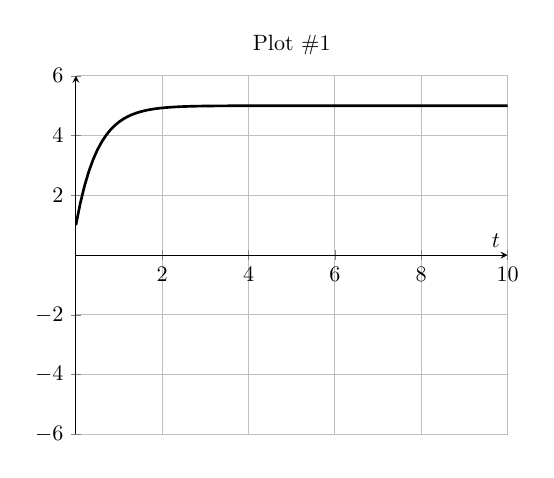
\begin{tikzpicture}[scale=\scl]
        \begin{axis}[axis lines=center, xlabel={$t$}, xmin=0, xmax=10, ymin=-6, ymax=6,
                grid, title={Plot \#1}]
                \addplot[very thick, domain=0:10, samples=100] {-4*exp(-2*x)+5};
        \end{axis}
    \end{tikzpicture}
    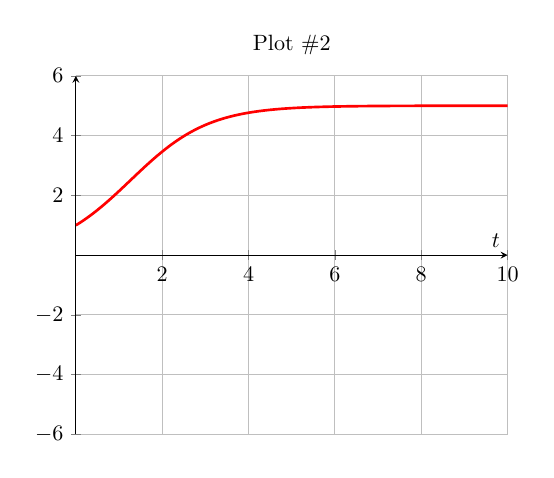
\begin{tikzpicture}[scale=\scl]
        \begin{axis}[axis lines=center, xlabel={$t$}, xmin=0, xmax=10, ymin=-6, ymax=6,
                grid, title={Plot \#2}]
                \addplot[very thick, domain=0:10, samples=150, color=red]
                {(5*exp(1.1*x))/(4+1*exp(1.1*x))};
        \end{axis}
    \end{tikzpicture}
\end{center}

\begin{center}
    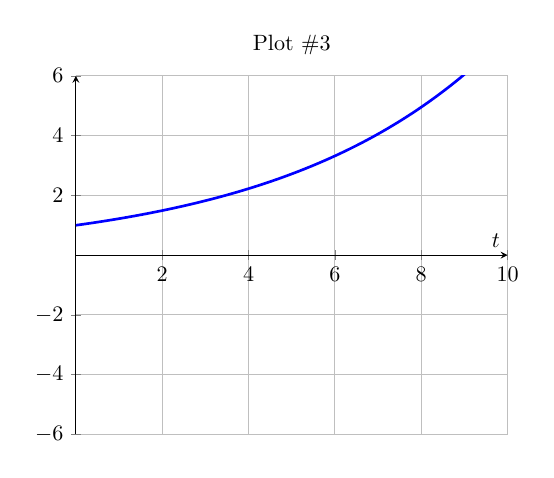
\begin{tikzpicture}[scale=\scl]
        \begin{axis}[axis lines=center, xlabel={$t$}, xmin=0, xmax=10, ymin=-6, ymax=6,
                grid, title={Plot \#3}]
                \addplot[very thick, domain=0:10, samples=100, color=blue] {exp(0.2*x)};
        \end{axis}
    \end{tikzpicture}
    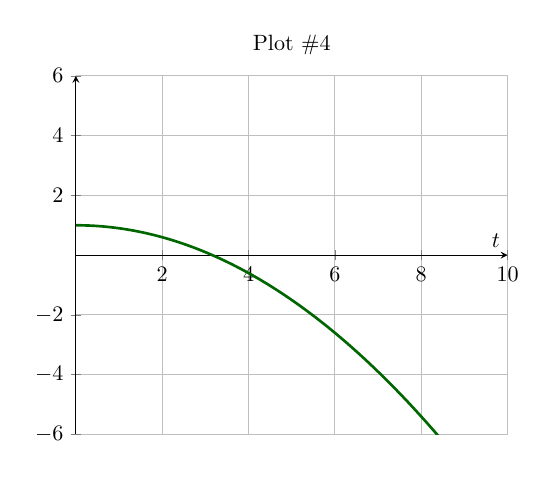
\begin{tikzpicture}[scale=\scl]
        \begin{axis}[axis lines=center, xlabel={$t$}, xmin=0, xmax=10, ymin=-6, ymax=6,
                grid, title={Plot \#4}]
                \addplot[very thick, domain=0:10, samples=100, color=green!40!black] {-0.1*x^2+1};
        \end{axis}
    \end{tikzpicture}
\end{center}
\end{problem}
\solution{
3,2,1,4. \\
Hint: Use what you know about the dynamics of the differential equations without solving
them.  For example, is there a steady state?  are there multiple steady states? etc.
}


\begin{problem}
    For each of the following scenarios write a differential equation and give an
appropriate initial condition.  Do not solve these differential
equations.
\begin{enumerate}
    \item[(a)] A tank contains 10kg of salt and 2000L of water.  Pure water enters the tank
    at a rate of 4L/min, the solution is thoroughly mixed, and solution is drained at 3
    L/min.  Let $S(t)$ be the amount of salt in the tank at time $t$.  Write a
    differential equation describing the amount of salt in the tank.
    \[ \frac{dS}{dt} = \underline{\hspace{2in}} \quad \text{with} \quad S(0) =
        \underline{\hspace{0.75in}} \]
        \solution{
            \[ \frac{dS}{dt} = -\frac{3S}{2000+1t} \quad \text{with} \quad S(0) = 10 \]
        }

    \item[(b)] Oil is pumped continuously from a well at a rate proportional to the amount
    of oil left in the well.  Initially there were 2 million barrels of oil in the well.
    Let $y(t)$ be the number is barrels left in the well (measured in millions of
    barrels).
    \vspace{0.1in} 
    \[ y' = \underline{\hspace{2in}} \quad \text{with} \quad y(0) =
        \underline{\hspace{0.75in}} \]
        \solution{
            $y'=-ky$ with $y(0) = 2$
        }
    \item[(c)] Newton's Law of Cooling states that the rate of change of the temperature
        of a cooling body (like tea in a cup) is proportional to the difference
        between the current temperature and the ambient room temperature.  Assume that the
        tea starts at 160$^\circ$F and cools, eventually, to 66$^\circ$F.  Write the
        differential equation associated with Newton's Law of Cooling.
        \[ \frac{dT}{dt} = \underline{\hspace{2in}} \quad \text{with} \quad T(0) =
            \underline{\hspace{0.75in}} \]
        \solution{
            \[ \frac{dT}{dt} = -k(T-66) \quad \text{with} \quad
                T(0) = 160 \]
        }
    \item[(d)] A pair of turtles, let's call them Adam and Eve, start a turtle colony in a
    small Montana pond (let's just ignore the lack of genetic diversity here).  The
    population of turtles in the pond follows these simple rules:  (1) If there
    are no turtles then the population clearly doesn't change, (2) the pond can support
    roughly 100 turtles, and (3) when the population is growing and is far away from the
    carrying capacity the growth rate is roughly proportional to the size of the
    population.  Let $P(t)$ be the size of the turtle population at time $t$.
    \[ \frac{dP}{dt} = \underline{\hspace{2in}} \quad \text{with} \quad S(0) =
        \underline{\hspace{0.75in}} \]
        \solution{
            \[ \frac{dP}{dt} = -kP\left( 1-\frac{P}{100} \right) \quad \text{with} \quad
                P(0) = 2 \]
        }

    \item[(e)] A 120-gallon tank initially contains 90 pounds of salt dissolved in 100
    gallons of water. Brine containing 2 pounds per gallon of salt flows into the tank at
    a rate of 4 gallons per minute and the well stirred mixture flows out of the tank at a
    rate of 3 gallons per minute (so the tank is filling up). Write a differential
    equation for the amount of salt in the tank.
    \[ \frac{dS}{dt} = \underline{\hspace{2in}} \quad \text{with} \quad S(0) =
        \underline{\hspace{0.75in}} \]
        \solution{
            \[ \frac{dS}{dt} = 8  -\frac{3S}{100+t} \quad \text{with} \quad y(0) = 10 \]
        }
\end{enumerate}
\end{problem}


\begin{problem}
    In Problem \ref{prob:ice_balls} we built models for the melting of ice cubes.  Solve
    both of the differential equations resulting from those models and answer the
    question: which type of ice cube will keep my drink colder longer.
\end{problem}
